% Created 2022-02-18 Fri 15:47
% Intended LaTeX compiler: pdflatex
\documentclass[presentation,aspectratio=1610]{beamer}
\usepackage[utf8]{inputenc}
\usepackage[T1]{fontenc}
\usepackage{graphicx}
\usepackage{grffile}
\usepackage{longtable}
\usepackage{wrapfig}
\usepackage{rotating}
\usepackage[normalem]{ulem}
\usepackage{amsmath}
\usepackage{textcomp}
\usepackage{amssymb}
\usepackage{capt-of}
\usepackage{hyperref}
\usepackage{khpreamble}
\usepackage{algorithm}
\usepackage{hyperref}
\usepackage{framed}
\usepackage[noend]{algpseudocode}
\usepackage{tikz,pgf}
\usetikzlibrary{shapes.geometric}
\newcommand{\sign}{\mathrm{sign}}
\renewcommand{\transp}{^{\mathrm{T}}}
\DeclareMathOperator*{\argmin}{arg\,min}
\DeclareMathOperator*{\argmax}{arg\,max}
\DeclareMathOperator*{\EXP}{E}
\DeclareMathOperator*{\COV}{cov}
\definecolor{uured}{rgb}{0.65, 0., 0.}
\DeclareMathOperator*{\E}{E}
\DeclareMathOperator*{\Var}{Var}
\usetheme{default}
\author{Kjartan Halvorsen}
\date{\today}
\title{Gazebo and ROS  - part 1}
\hypersetup{
 pdfauthor={Kjartan Halvorsen},
 pdftitle={Gazebo and ROS  - part 1},
 pdfkeywords={},
 pdfsubject={},
 pdfcreator={Emacs 26.3 (Org mode 9.4.6)}, 
 pdflang={English}}
\begin{document}

\maketitle

\section{Introduction}
\label{sec:org2109fbd}

\begin{frame}[label={sec:orge30a877}]{Sources}
\begin{itemize}
\item \url{http://gazebosim.org/}
\item \url{http://gazebosim.org/tutorials/?tut=ros\_comm}
\item \url{http://sdformat.org/}
\item \url{http://docs.ros.org/kinetic/api/gazebo\_msgs/html/index-msg.html}
\end{itemize}
\end{frame}

\begin{frame}[label={sec:orgf77e2fd}]{What is Gazebo?}
A 3D simulation and visualization environment containing a physics engine.
\end{frame}

\begin{frame}[label={sec:org45cd4bc}]{Why use Gazebo?}
It is a playground for your robot where you can test \alert{actuators}, \alert{sensors} and \alert{control algorithms}.
\end{frame}

\begin{frame}[label={sec:org20f4007},fragile]{Let's start with a fun example}
 Start \texttt{roscore}, \texttt{gazebo} and \texttt{gazebo\_ros} in two separate terminals.

\begin{block}{Terminal 1}
\begin{verbatim}
~$ roscore 
\end{verbatim}
\end{block}

\begin{block}{Terminal 2}
\begin{verbatim}
~$ rosrun gazebo_ros gazebo
\end{verbatim}
\end{block}
\end{frame}

\begin{frame}[label={sec:org4d8c487}]{What just happened}
\begin{center}
\begin{tikzpicture}
 \node (gazebo) {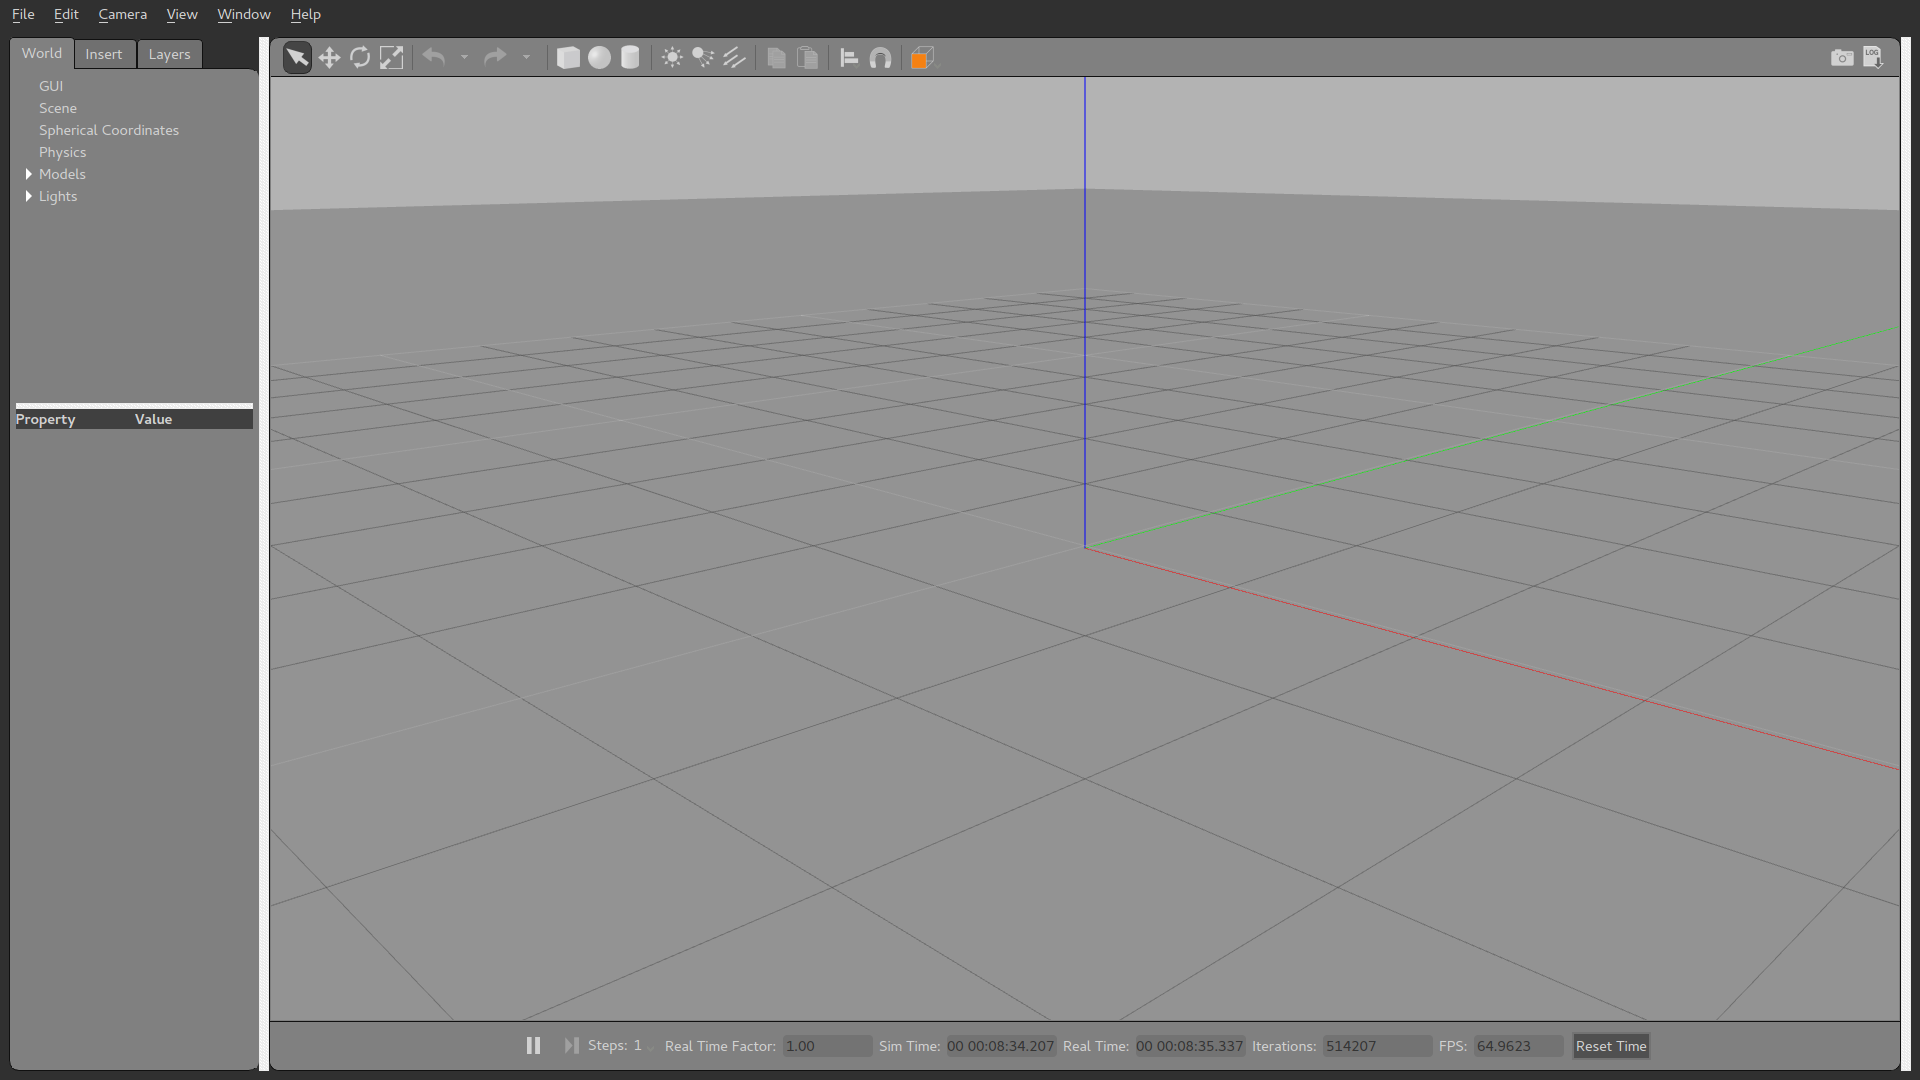
\includegraphics[width=45mm]{gazebo-gui-empty.png}};
 \node[ellipse, draw, 
       minimum height=15mm, minimum width=20mm, maximum width=22mm, right of=gazebo, 
       node distance=7cm, text align=center] (gnode) {gazebo ros node};

\node[coordinate, right of=gnode, node distance=3cm] (tmp) {};
\node[above of=tmp, node distance=3cm] (topics) {
\includegraphics[width=25mm]{chalkboard.png}};
\node[below of=tmp, node distance=3cm] (services) {
\includegraphics[width=25mm]{chalkboard.png}};
\node[white, above of=tmp, node distance=35mm] {Topics};
\node[white, below of=tmp, node distance=25mm] {Services};

\draw[<->, thick] (gazebo) -- node[above] {Gazebo comm} (gnode);
\draw[<->, thick] (gnode) -- node[left] {ROS comm} (topics);
\draw[<-, thick] (gnode) -- node[left] {ROS comm} (services);

\end{tikzpicture}
\end{center}
\end{frame}
\begin{frame}[label={sec:org57ea2f4},fragile]{Add some junk to the world}
 \begin{verbatim}
~$ rosrun gazebo_ros spawn_model -database coke_can \
> -sdf -model coke_can1 -y 1 -x 0
~$ rosrun gazebo_ros spawn_model -database coke_can \
> -sdf -model coke_can2 -y 2 -x 0
\end{verbatim}
\end{frame}

\begin{frame}[label={sec:org1147631},fragile]{See the physics engine in action}
 Pause the gazebo physics engine, then lift the first can up 50cm
\begin{verbatim}
~$ rosservice call /gazebo/pause_physics
~$ rosservice call /gazebo/set_model_state \ 
> '{model_state: { model_name: coke_can1, \
> pose: { position: { x: 0., y: 1. ,z: 0.5 } }, \
> reference_frame: world } }'
\end{verbatim}

and drop the can (start simulation in the gazebo gui)!
\end{frame}

\begin{frame}[label={sec:org660c744}]{On your own: Drop the first can on top of the second can from two meters}
\end{frame}

\section{Gazebo\textsubscript{ros} fundamentals}
\label{sec:org8aa7a76}

\begin{frame}[label={sec:org3804781},fragile]{Gazebo published topics}
 Which of the following topics are \alert{not} available?

\begin{verbatim}
/clock
/gazebo/link_states
/gazebo/model_states
/gazebo/parameter_descriptions
/gazebo/parameter_updates
/gazebo/set_link_state
/gazebo/set_model_state
/gazebo/set_world_state
/rosout
/rosout_agg
\end{verbatim}
\end{frame}

\begin{frame}[label={sec:org3c56421},fragile]{Gazebo services provided}
 Which of the following services are \alert{not} available?
\begin{verbatim}
/gazebo/apply_body_wrench
/gazebo/clear_joint_forces
/gazebo/get_joint_properties
/gazebo/set_joint_force
\end{verbatim}

Hint: \texttt{rosservice}
\end{frame}

\begin{frame}[label={sec:org445ccf1},fragile]{Getting the coke can airborn}
 We can apply a \alert{wrench} ( a force and torque pair) to any rigid body in the gazebo world

\begin{verbatim}
~$ rosservice info /gazebo/apply_body_wrench
\end{verbatim}

What arguments does the service take?
\end{frame}

\begin{frame}[label={sec:org5143ecb}]{Getting the coke can airborn, contd}
If the can has a vertical launch velocity of \(\unit{v_L}{\meter\per\second}\), it will reach a height where its potential energy is the same as the kinetic energy at launch. So to reach a height of \(h=\unit{3}{m}\) we need a launch velocity of
\[ v_L = \]
\end{frame}

\begin{frame}[label={sec:orga352c4e}]{Getting the coke can airborn, contd}
If the can has a vertical launch velocity of \(\unit{v_L}{\meter\per\second}\), it will reach a height where its potential energy is the same as the kinetic energy at launch. So, to reach a height of \(h=\unit{3}{m}\) we need a launch velocity of
\[ v_L = \sqrt{2gh} \approx \unit{7.7}{\meter\per\second}\]
\end{frame}

\begin{frame}[label={sec:org7f697b6}]{Kicking the coke can, theory}
Let's apply a constant, large force \(F=F_v+mg\) under a short time \(\tau=\unit{10}{\milli\second}\). Newton's second law gives
\[ \frac{d}{dt} (mv) = F_v + mg - mg \]

\[ \int_0^\tau (\frac{d}{dt} mv) dt = \int_0^\tau F_v dt\]
\pause
\[ mv_L - 0 = F_v \tau \]
The coke can has a mass of \(m=\unit{0.39}{\kilo\gram}\). What force \(F_v\) is needed?
\end{frame}


\begin{frame}[label={sec:org59f5f32},fragile]{Kicking the coke can, for real (sort of)}
 \begin{verbatim}
~$ rosservice call /gazebo/pause_physics
~$ rosservice call /gazebo/apply_body_wrench \
> '{body_name: "coke_can2::link" , \ 
> wrench: { force: { z: 300 } }, duration: 10000000 }'
\end{verbatim}
\end{frame}


\section{Introduce our own design}
\label{sec:org696fad6}
\begin{frame}[label={sec:orgbfc8910}]{URDF - Unified Robotic Description Format}
Defining a robot

\href{https://youtu.be/pT5iQaG9aVU}{Video}
\end{frame}

\begin{frame}[label={sec:org41e34b2},fragile]{Spawning a model defined by a urdf file}
 \begin{verbatim}
~$ rosrun gazebo_ros spawn_model -file ./furuta.urd -urdf -\
>   y 2 -model furuta
\end{verbatim}
\end{frame}
\begin{frame}[label={sec:orgccedc16},fragile]{Making the model move}
 \begin{verbatim}
~$ rosservice call /gazebo/apply_joint_effort \
"joint_name: 'furuta::base_to_one_prox' effort: 10 duration: 10000000"
\end{verbatim}
\end{frame}
\end{document}